\chapter{Results}
\label{results}
In this chapter we present the results of our approach in every important part of our work. We are going to describe through examples and test results what we have achieved in the motion part, in the communication part, in the coordination part and finally and the most important the overall results which are obtained from real competitive soccer matches against other teams who have participated in at least one time at RoboCup 3D Simulation League in the past.


\section{Motion}
This section presents the improvements we have accomplished to achieve in the motion part of our agent. In general, as we described in motion Section~\ref{Motions} , motion files are generated by other teams or other platforms such as FIIT project or Webots Simulator. We can only optimize these motions through several tests. Optimization of these motions, make motion part of our player skills to reach an adequate level. Table~\ref{MotionImprovements} presents the improvements made in motions only in cases that it was possible. Optimized walk motion has reached a speed up to .45m/s which is comparable but much slower than the UT Austin Villa's walking engine which produces a walk motion of .71m/s. Furthermore strong kick movement has reached a 5.5 meters range in just 2.5 seconds of execution. Turn motion is using Webots motion files. Turning which has reached to a speed up to 30 degrees per second. 

\begin{table}[t!]
\caption{Motion's Performance Improvement (Averaged Speeds and Ranges)}
\label{MotionImprovements}
\begin{center}
\begin{small}
\begin{tabular}{ccccc}
\textbf{Motion Version} & \textbf{Walk(m/s)}	& \textbf{Turn(d/s)}	& \textbf{Kick(m)}&\textbf{Strong Kick(m)} \\
\midrule
Webots (Text-Based) 		& 0.11 				& 21 				& 3 				& - \\
FIIT (XML)				& 0.22 				& 25 				& 3 (4 Sec.) 		& 4 (5 Sec.) \\
\textbf{AST\_3D} 		& 0.45 	& 30 		& 3 (2.5 Sec.)& 5.5 (2.5 Sec.) \\
\end{tabular}
\end{small}
\end{center}
\end{table}




\section{Communication}
Testing communication process through ideal external communication, when only our team has the ability to send messages achieved good results. Agents were able to ``hear'' all their teammates in an averaged 24 simulation cycles. In addition, even in real matches conditions when both teams had the ability to send messages to their teammates the results remained approximately the same. Table~\ref{CommunicationResults} presents the performance of each communication phase during coordination process. We can realize that there are not serious delays in these communication phases. This happens due to the fact soccer simulation server does not allow players to send messages in the same server cycle. We take advantage of the fact that there are separately tracked capacities for both teams, sending our messages only in labeled timed slices we ensure that opponent team will not able to block our messages even in extreme conditions when opponents shout messages constantly. The only case that our team is exposed in opponents broadcasting is when opponents choose the same time slices (cycles), as we do, to shout their messages.

\begin{table}[b!]
\caption{Communication Results in Ideal and Match Conditions}
\label{CommunicationResults}
\begin{center}
\begin{small}
    \begin{tabular}{ccc}
    \textbf{Communication Phase} 	& \textbf{Ideal (Cycles (Sec.))}			& \textbf{During Match (Cycles (Sec.))} \\
    \midrule
    Init Messages 					& 24  ( 0.48 ) 			& 24 	( 0.48 )		\\
    Coordination Messages			& 24  ( 0.48 )			& 42.5  ( 0.85 )		\\
    Action Messages 				    & 24  ( 0.48 )			& 24 ( 0.48 )	 		\\
    \end{tabular}
    \end{small}
\end{center}
\end{table}





\section{Goalkeeper}
To determine his ability to stop or to delay seriously opponents from scoring, we ran several tests in three different conditions. In these three tests, players other  than goalkeeper did not take part.
First, we did not use a goalkeeper, allowing our opponents to reach our goal without any obstacle in their way. Opponents team managed to score an averaged of seven goals in this case.
Next, we used an agent as the goalkeeper but with an ``empty'' behavior with which he was not able to perform any motion or to track the ball, standing useless and still at the center of our goal. Opponents team managed to score equal amount of goal with (No Goalkeeper) test.
In our final test, we used a goakeeper which made use of its current behavior developed by us. We achieved in reducing conceded goal from seven to three. Table~\ref{GoalKeeperResults} presents these results.



\begin{table}[t!]
\caption{Goalkeeper Averaged Results in Half-Games.}
\label{GoalKeeperResults}
\begin{center}
\begin{small}
    \begin{tabular}{cc}
    \textbf{GoalKeeper Type} 	& \textbf{Goals Conceded}\\
    \midrule
    No Goalkeeper						& 7\\
    Goalkeeper, ``Empty'' Behavior	& 7\\
    Goalkeeper, ``Full'' Behavior	& 3\\
    \end{tabular}
    \end{small}
\end{center}
\end{table}


\section{Coordination}

\subsubsection*{Coordination Beliefs Update}
As we have mentioned before in this thesis (cf. Section~\ref{sec:UpdateBeliefs}), coordination beliefs are very important in order for coordinator to have an adequate knowledge of the world state. Most of functionalities of the coordination protocol are depended on these beliefs.
Most important of these beliefs is the estimation about the position of the ball. Estimation derived by weighted observation sets gave nice results. Figure~\ref{} presents the estimated position of the ball (blue circle) in several examples. Recall, that every observation set has a distance threshold; these thresholds are defined in the corresponding figures with a cyan and red circle. Observation sets depicted with a red circle imply that they have more that one observation in them. On the other hand cyan ones include only one observation. The white circles having small radii, represent individual observations coming from agents.

\begin{figure}[h!]
\centering
  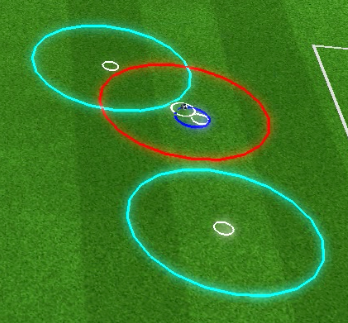
\includegraphics[height=6cm,width=6cm]{Chapter5/figures/BallObs1.png}\	
  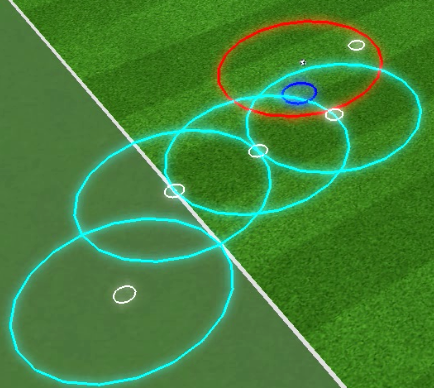
\includegraphics[height=6cm,width=6cm]{Chapter5/figures/BallObs2.png}\\
  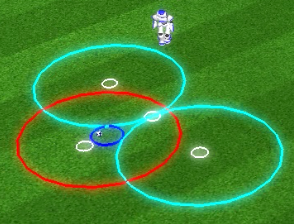
\includegraphics[height=6cm,width=6cm]{Chapter5/figures/BallObs3.png}\	
  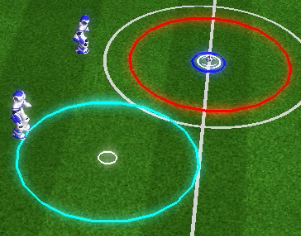
\includegraphics[height=6cm,width=6cm]{Chapter5/figures/BallObs4.png}
  \caption{Estimated Position of the Ball in Four Examples.} 
  \label{fig:AttackingPositioning1}
\end{figure}



\subsubsection*{Coordination Achievements}
Coordination is the most significant part in this thesis. As we have presented in Chapter~\ref{Coordination} of this thesis, coordination is responsible for assigning roles to the players, finding strategic positions, computing optimal mappings among players and positions. We have discussed every aspect of this procedure and now we present the results of this dynamic procedure. Coordination, expectedly, gave very good results. In a dynamic environment like this, in which there is a big need for dynamic coordination and cooperation among the agents we achieved 
to create a coordination system which has several advantages over other coordination systems with more static approaches. Some of the most important advantages of our coordination protocol is described below.

\begin{description}
\item[Offensive Positioning]
Finding and assigning worthy positions to the agents while our team is in an offensive situation was a main goal of our positioning system. In every occasion in which an agent of our team has the ball in its possession, Active agents are assigned optimal positions according to a specific evaluation method to support the on ball player. Figure~\ref{fig:AttackingPositioning1} presents an example of this positioning system. As we can realize, active players are given routes to follow to be close to the opponents' goal, seeking to exploit any arising opportunity to score a goal. Figure~\ref{fig:AttackingPositioning2} presents another example, a possible shoot by the on ball player will give active agents the chance to score a goal.


\begin{figure}[h!]
\centering
  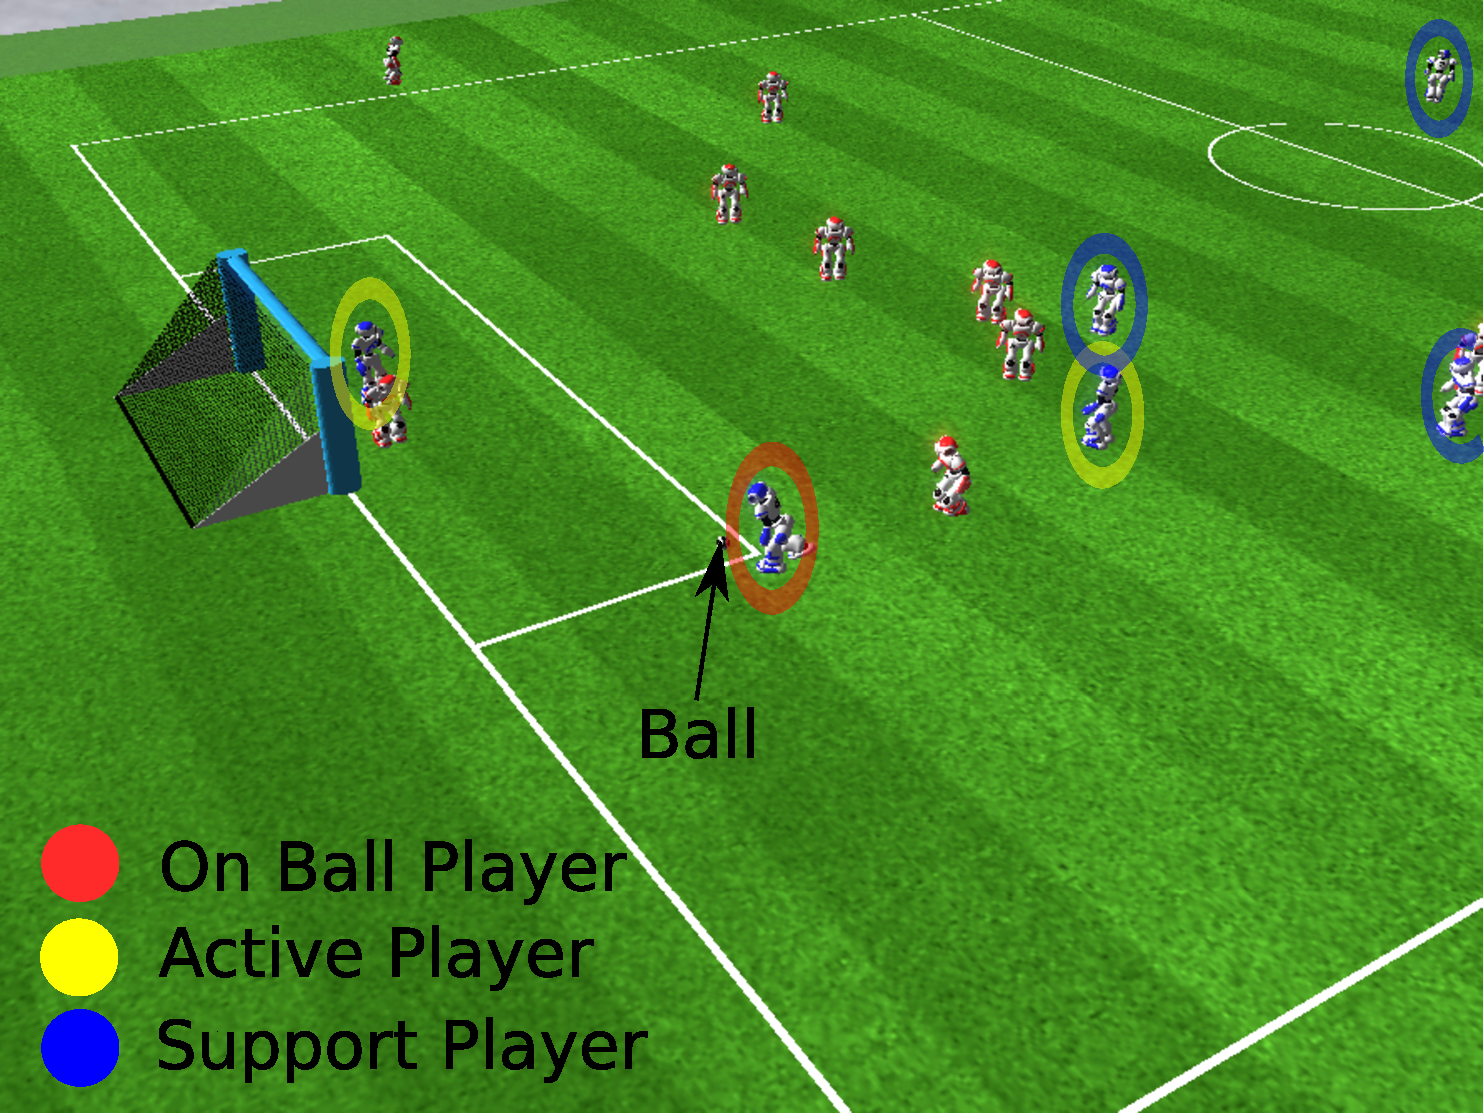
\includegraphics[width=0.6\textwidth]{Chapter5/figures/3.pdf}\\
  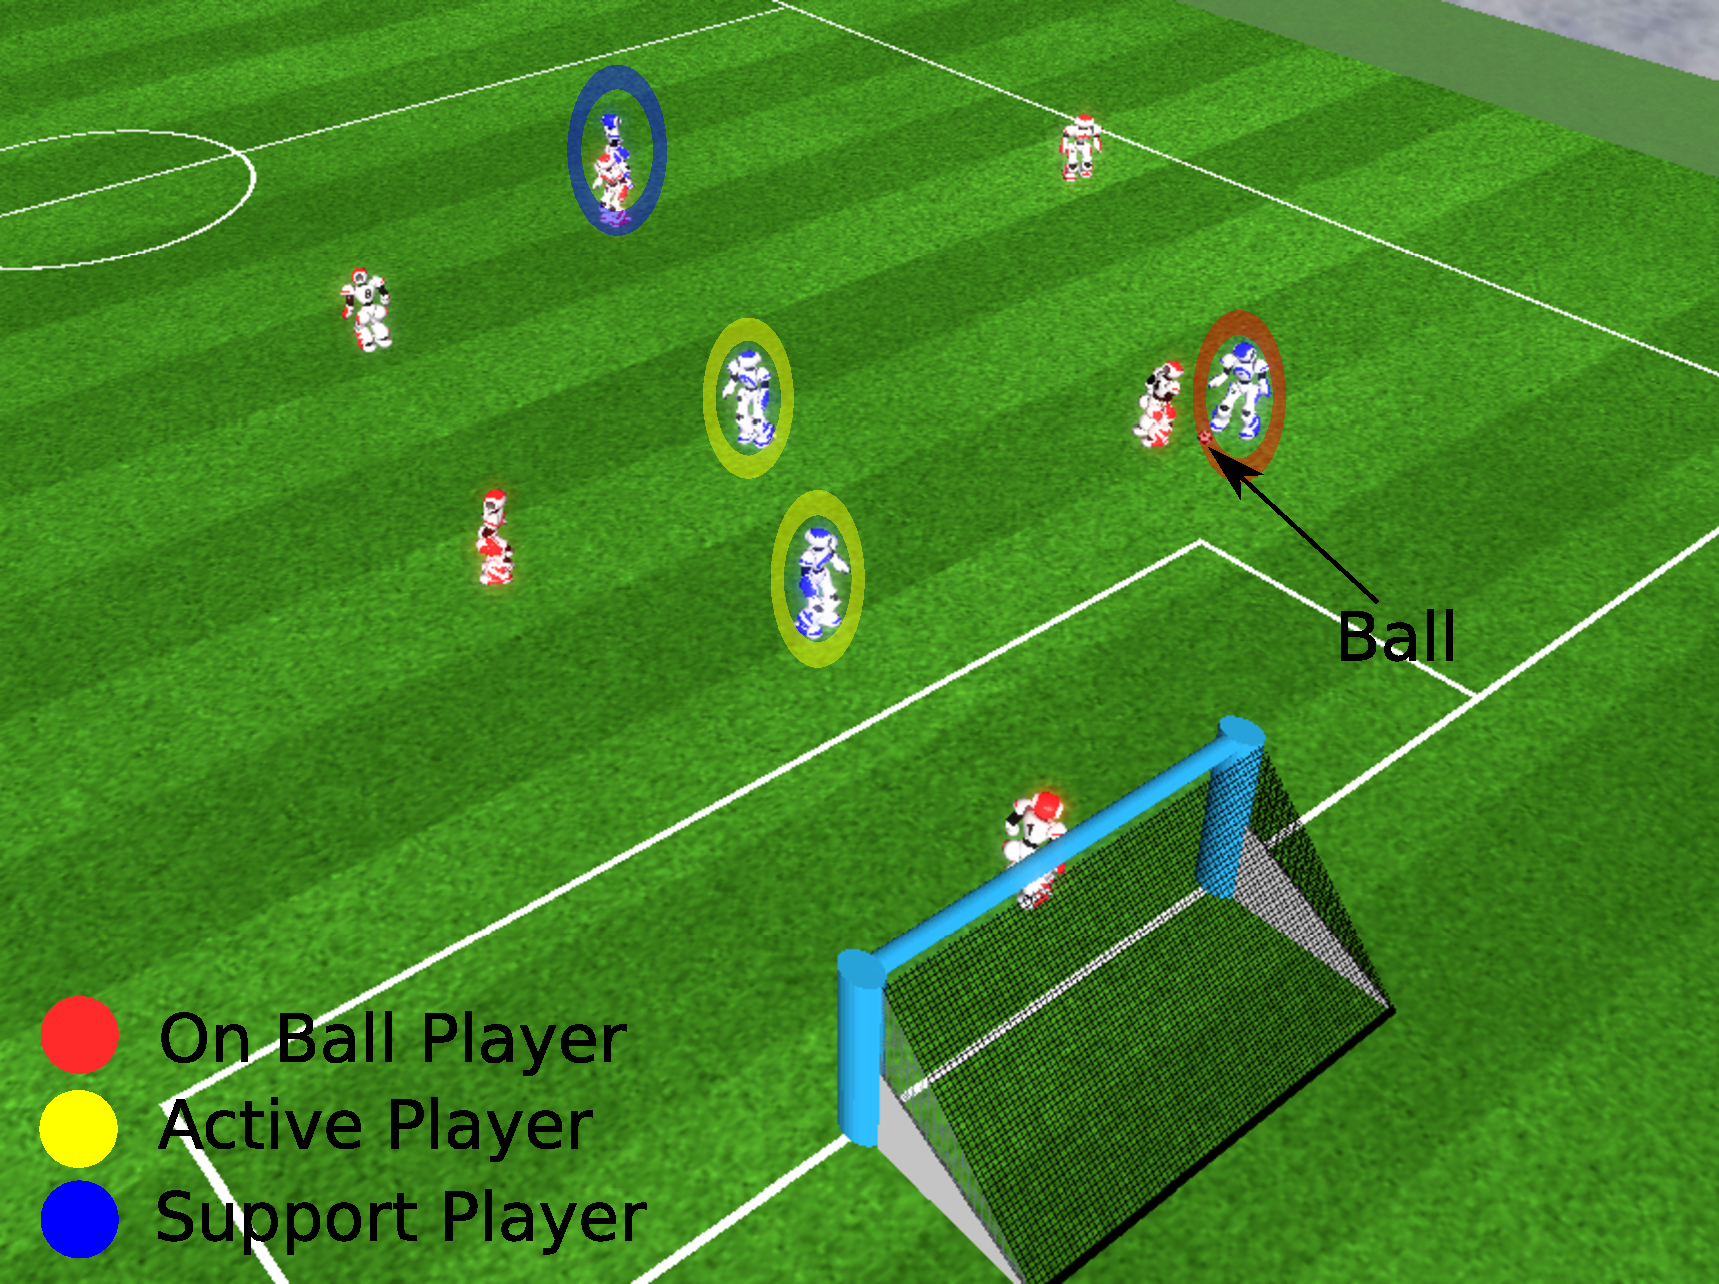
\includegraphics[width=0.6\textwidth]{Chapter5/figures/5.pdf}
  \caption{Offensive Positioning Resulting by Coordination Protocol, Example 1.} 
  \label{fig:AttackingPositioning1}
\end{figure}

\clearpage



\item[Defensive Positioning]
Finding and assigning positions to the agents while our team was in a defensive situation was another main target of our positioning system. In every occasion, in which our team is on a defensive role in the field, active agents are assigned worthy positions to support the on ball player and protect possible opponent's strike towards our goal. As we can realize, active players are assigned positions in the field which are proven disastrous for the opponents. Figures~\ref{fig:DefendingPositioning},~\ref{fig:DefendingPositioning1} presents two examples of the defending positioning system, Active players have blocked in both cases the opponent agent's way to our goal.


\begin{figure}[t!]
\centering
  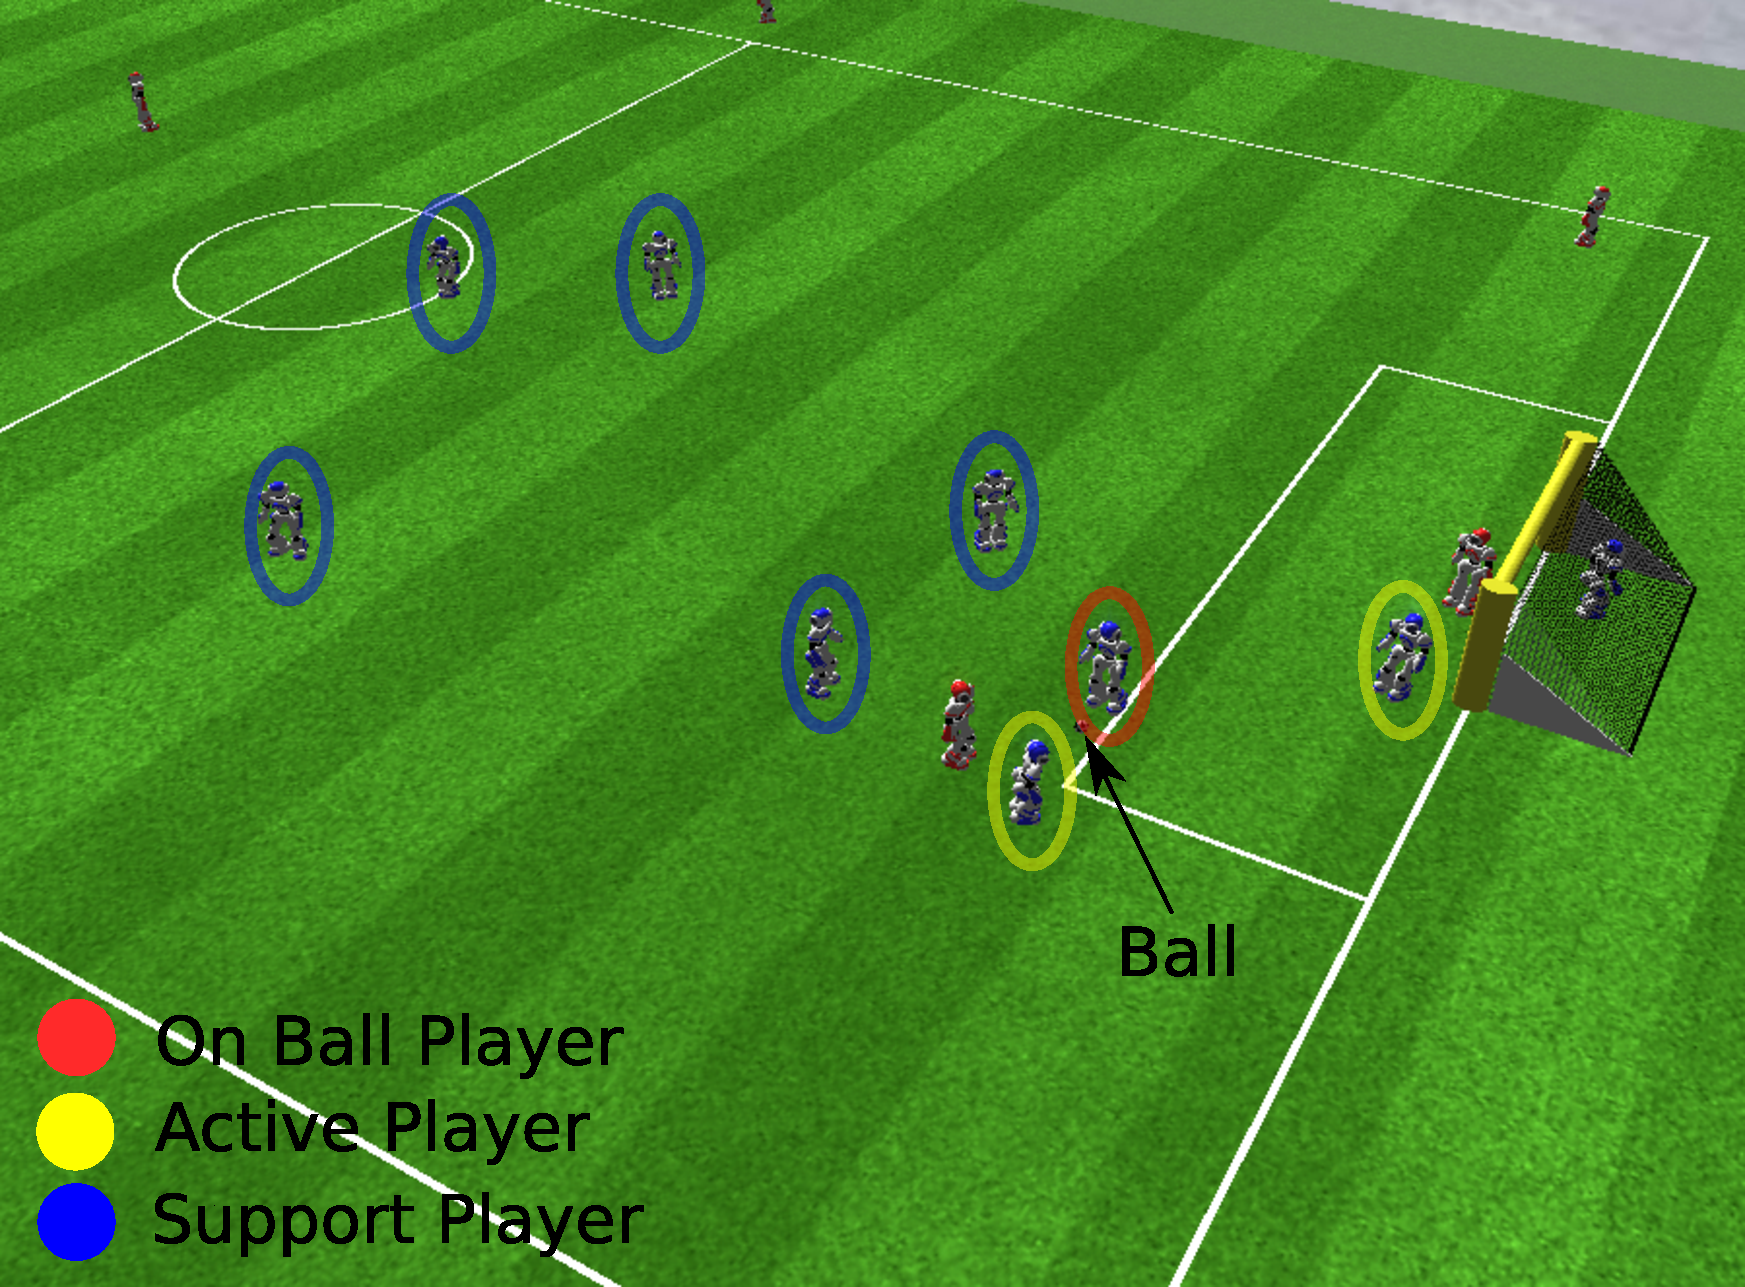
\includegraphics[width=0.8\textwidth]{Chapter5/figures/1.pdf}
  \caption{Defensive Positioning Resulting by Coordination Protocol, Example 1.} 
  \label{fig:DefendingPositioning}
\end{figure}


\begin{figure}[t!]
\centering
  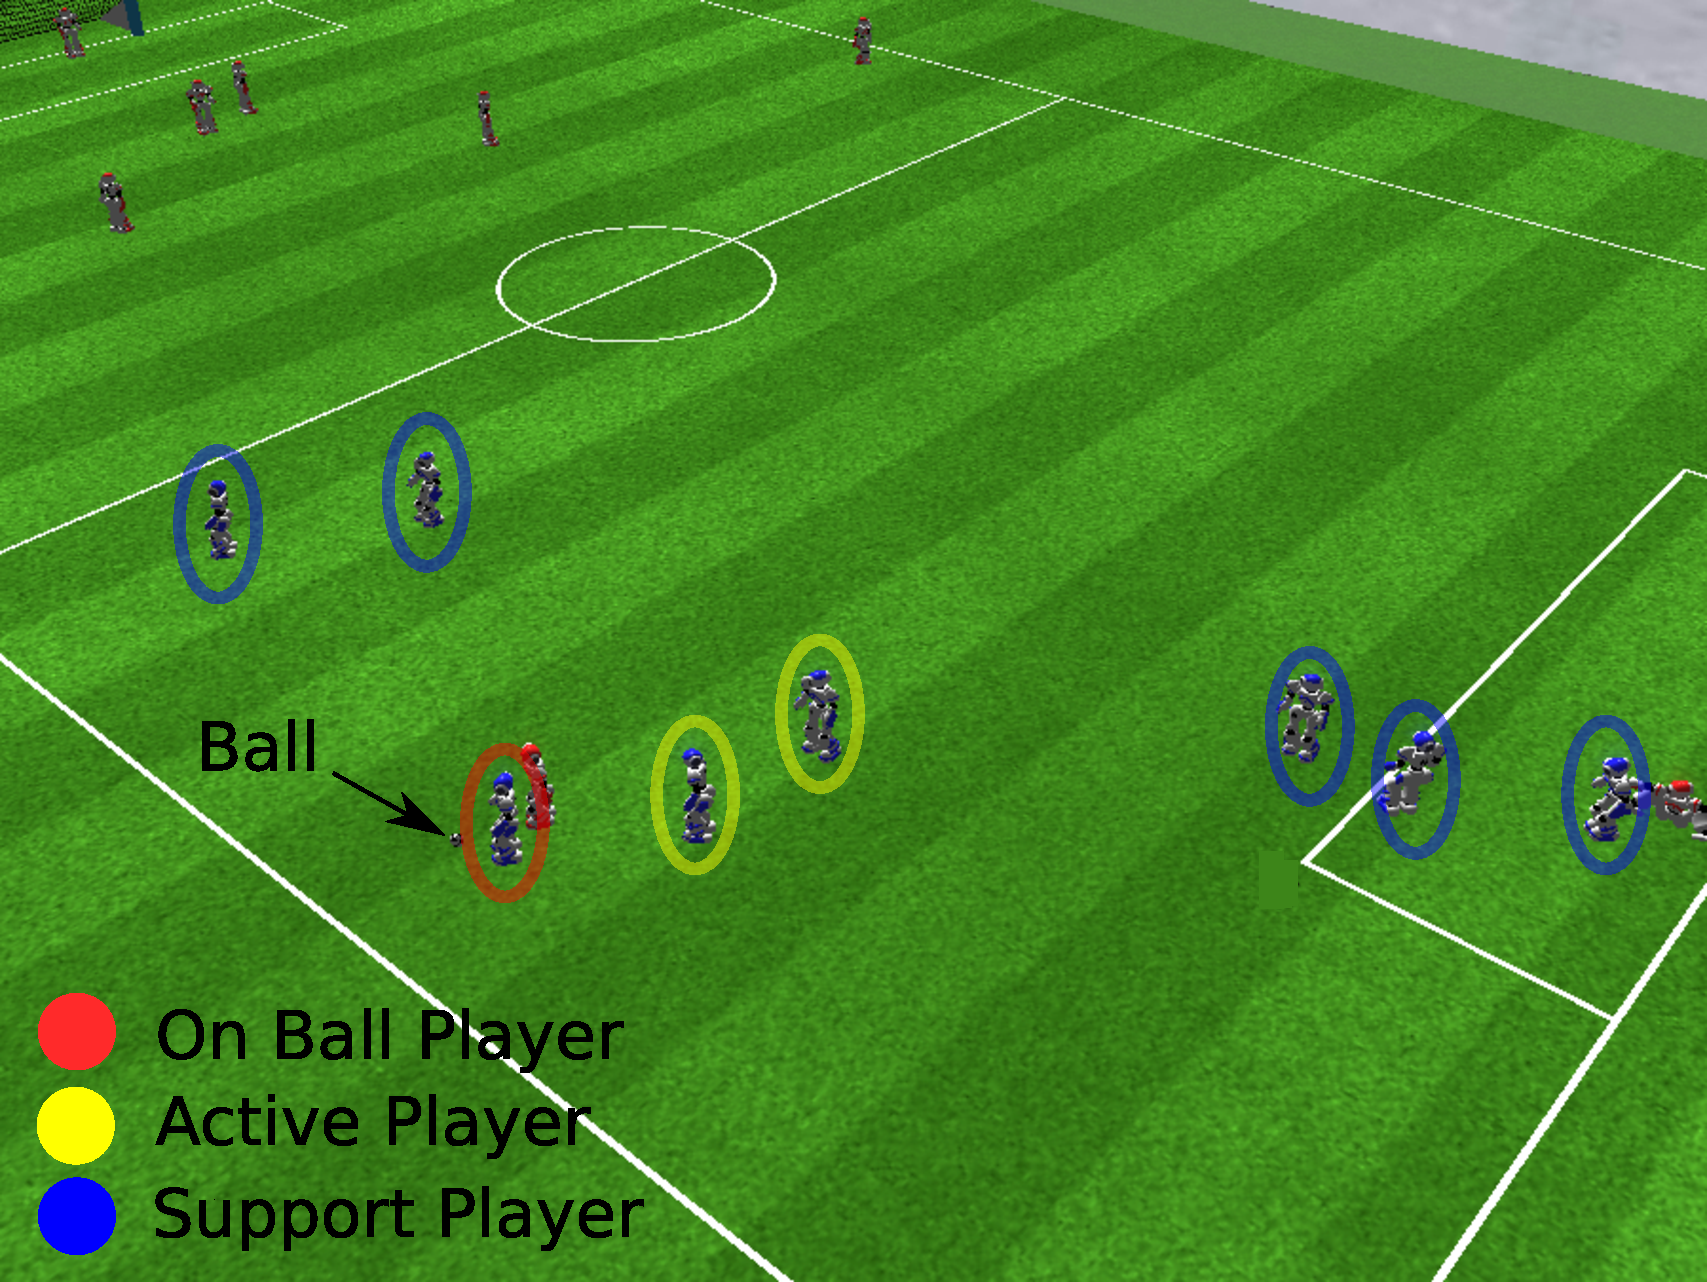
\includegraphics[width=0.8\textwidth]{Chapter5/figures/2.pdf}
  \caption{Defensive Positioning Resulting by Coordination Protocol, Example 2.} 
  \label{fig:DefendingPositioning1}
\end{figure}

\item[Formation Consistency]
Dynamic role assignment was one of the most significant parts of our team coordination system. In many occasions during game-play we have seen too many times agents changing roles and duties with each other. Team coordination system was built for that, to be adaptable in different situations inside a mostly dynamic environment like robotic soccer. This function resulting our team to have an adequate role distribution in every moment within a simulation soccer game. Agents are assigned roles which are proven to be worthy and costless in terms of the overall movement of our team into the soccer field. Figure~\ref{fig:StrategicPositioning} presents how this advantage of our coordination protocol depicted in the soccer field during game time. Active agents, as well as, on ball player are assigned specific roles from the available team formation roles. Remaining roles are available to be assigned to other players. Each one of the agents in blue circle is assigned a specific role which is described. For every given time in a soccer match our team will follow this property, resulting to a well placed team in the field, where all agents are going to have positions which are worthy and reasonable towards soccer variables.

\begin{figure}[t!]
\centering
  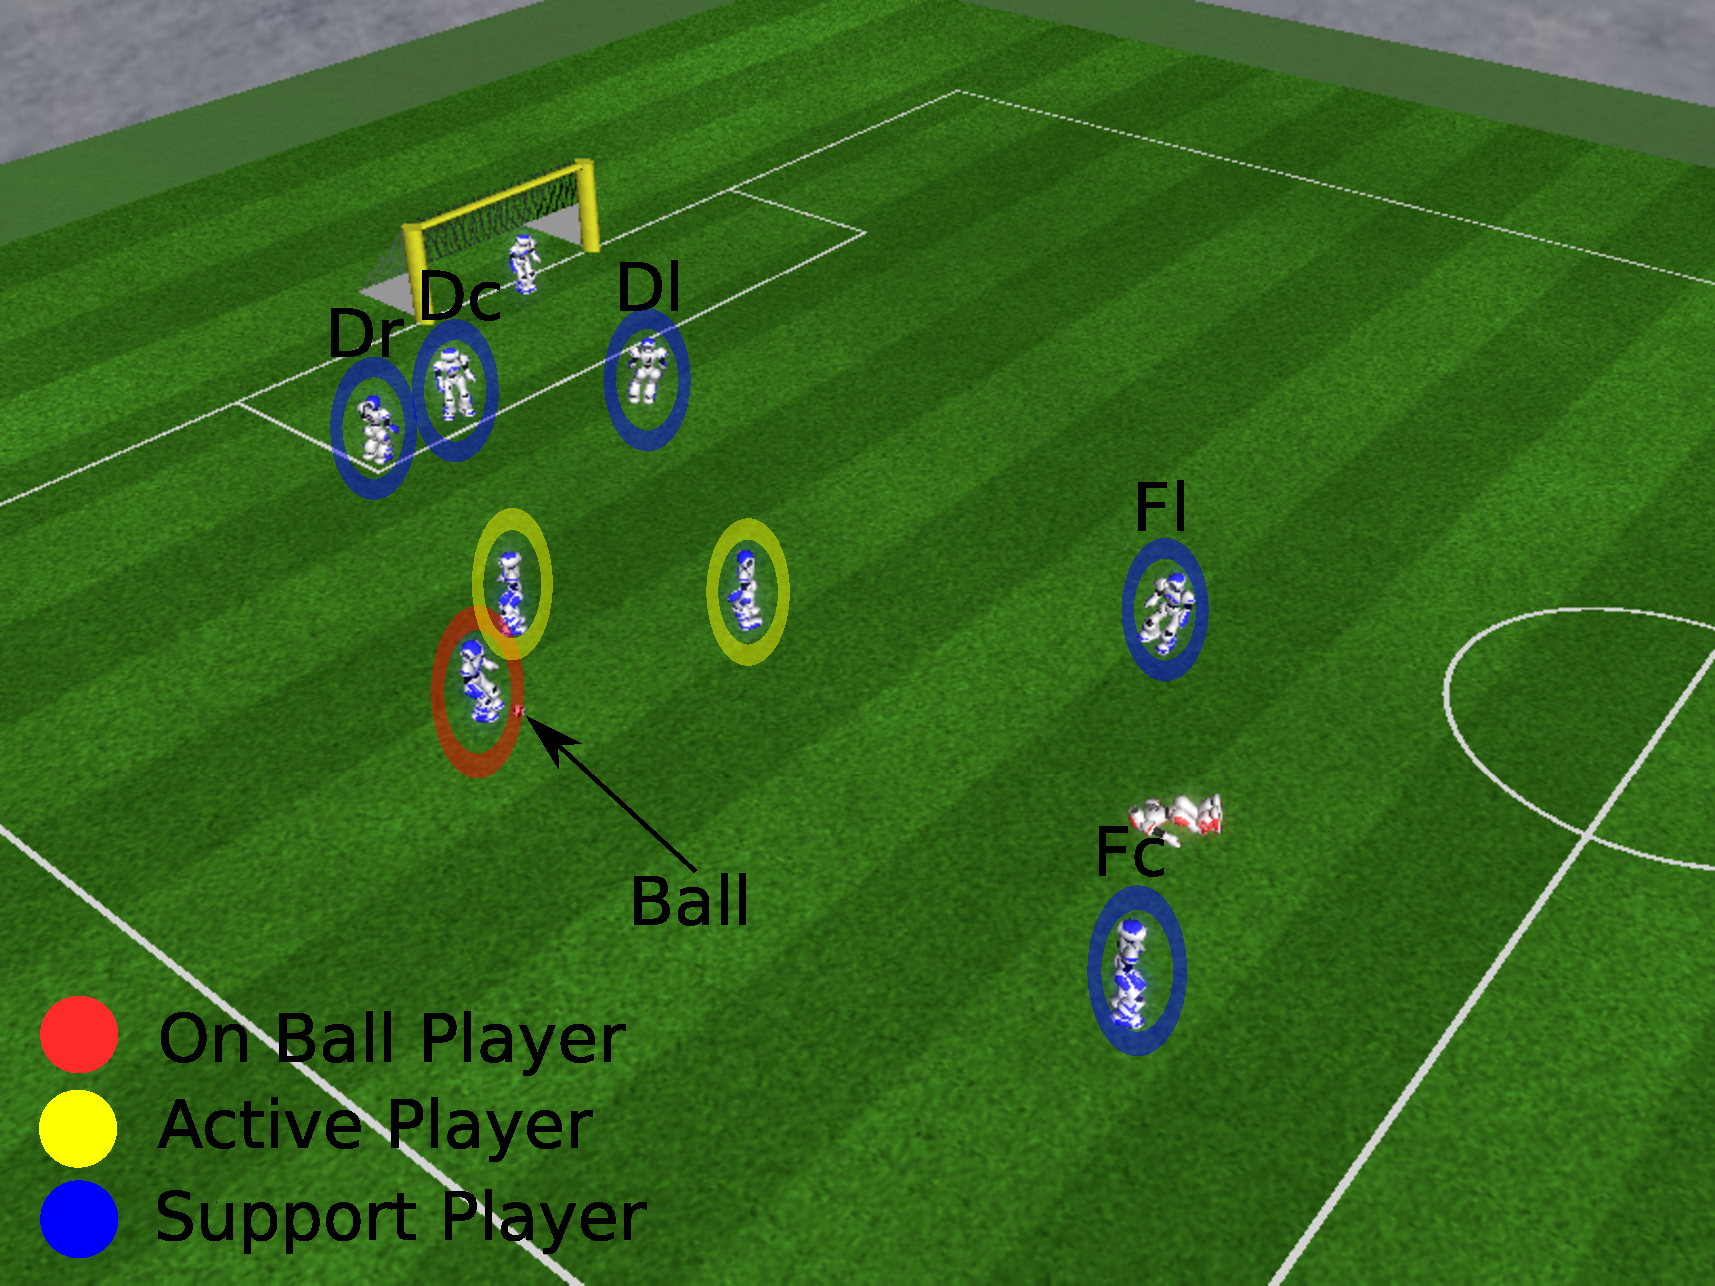
\includegraphics[width=0.8\textwidth]{Chapter5/figures/4.pdf}
  \caption{Formation Consistency Resulting by Coordination Process Via Team Roles Assignment.} 
  \label{fig:StrategicPositioning}
\end{figure}

\end{description}

\clearpage


\section{Games}
Finally, in order to test our created team in the most realistic way. We decide to test our team in real conditions playing against teams that have already participated in RoboCup 3D Soccer Simulation League. We have selected nine teams from the competition held in Istanbul, 2011 and one team (MAK) from Iran open, 2011. These teams are:
\begin{description}
\item[RoboCanes]	University of Miami, USA 
\item[UT Austin Villa]	University of Texas at Austin, USA
\item[NomoFC]	Osaka University, Japan
\item[OxBlue]	University of Oxford, UK
\item[L3MSIM]	Paris8 University,France
\item[Kaveh] 	Shahid Rajaee University, Iran University of Science and Technology, Iran
\item[beeStanbul]	Istanbul Technical University, Turkey
\item[Farzanegan]	Farzanegan high school, Iran
\item[MAK]	Ehsan Mosavi, University Of Kerman Mehravaran ,3D Robotics, Iran
\item[FUTK3D]	Fukui University of Technology, Japan
\end{description}

\subsubsection*{Individual Games}

\begin{table}[t!]
\caption{All Played Games Results}
\label{GameResults}
\begin{center}
    \begin{tabular}{cccccc}
    \textbf{Team} 	& \textbf{W} & \textbf{D} & \textbf{L} & \textbf{AGD}\footnotemark 	& \textbf{Games}   \\
    \midrule
    UTAustinVilla 	& 0		& 0		& 4		& -5.2		& 4 			\\
    Robocanes 		& 0		& 0		& 1		& -6.0		& 1 			\\
    BeeStanbul		& 0		& 0		& 3		& -4.0		& 3				\\
    NomoFC 			& 1		& 2		& 0		& +0.3 		& 3 			\\
    Rail 			& 0		& 4		& 0		& 0.0 		& 4 			\\
    OxBlue 			& 0		& 0		& 2		& -1.5 		& 2 			\\
    FUTK3D 			& 0		& 5		& 0		& 0.0 		& 5 			\\
    FARZANEGAN 		& 1		& 1		& 0		& +0.5 		& 2 			\\
    MAK 		    & 2		& 0		& 0		& +2.0 		& 2 			\\
    L3M-SIM			& 3		& 2   	& 0		& +0.6 		& 5 			\\     
    \end{tabular}
\end{center}
\end{table}



Playing against these teams, most of these have participated into one or more Robocup competitions, we have gained a lot of experience and we have seen how our team and especially our coordination protocol functions in different situations in a such dynamic environment. Due to lack of dynamic motions, our agents have poor movement especially in comparison with the Simulation league's best teams. However, we were able to perform well and score some goals against weaker teams of this competition.

After all these test-matches against teams who have participated into one or more Robocup competitions, we have gained a lot of experience and we have seen how our team reacts in different situations in such a dynamic environment. Due to lack of dynamic motions, our agents has poor movement especially in comparison with the RoboCup Simulation league's best teams. However, we were able to perform well and score some goals against weaker teams of this competition.

All executable binaries from teams are from previous events binaries, [Available online: \url{http://simspark.sourceforge.net/binaries/RoboCup2011/}]. All games had 10 minutes duration, same as real competition matches in official Robocup competition. Server and monitor were running in the same machine\footnotemark. Each one of the teams binaries was running in a separate machine\footnotemark . Table~\ref{GameResults} presents the results between our team and opponent teams. There is information about the average goal difference, the number of wins, the number of draws, the number of loses, and the total number of games we played with each team.
\footnotetext[1]{AGD: Averaged Goal Difference}
\footnotetext[2]{\textbf{Server}: Intel Core 2 Duo 3.16 Ghz, 5.8GiB Ram}
\footnotetext[3]{\textbf{Client1}: Intel Core 2 Duo 1.86 Ghz, 2GiB Ram}
\footnotetext[3]{\textbf{Client2}: Intel Quad Core i5 3.3 Ghz,4GiB Ram}
\clearpage


\subsubsection*{Mini Tournament}

Finally, we held a mini tournament in which teams participated in it were selected in order to have a competitive and in equal terms competition. Table~\ref{EasyTournament} presents the result table of this tournament. Win: 3 points, draw: 1 points, loss: 0 points.

\begin{table}[t!]
\caption{Mini Tournament (Tournament not completed yet)}
\label{EasyTournament}
\begin{center}
\begin{tabular}{l*{6}{c}r}
Team              	& P & W & D & L & F  & A & Pts \\ \hline
\textbf{AST3D} 		& \textbf{8} & \textbf{2} & \textbf{6} & \textbf{0} & \textbf{ 2} & \textbf{0} &  \textbf{12}  \\
NomoFC            	& 2 & 0 & 1 & 1 &  0 & 1 &  1  \\
L3M-SIM     		& 2 & 0 & 1 & 1 &  0 & 1 &  1  \\
Rail     		    & 2 & 0 & 2 & 0 &  0 & 0 &  2  \\
farzanegan     		& 2 & 0 & 2 & 0 &  0 & 0 &  2  \\
\end{tabular}
\end{center}
\end{table}






